\chapter{Системийн шаардлага}
\label{chapter3}
\section{Системийн дотоод үйл ажиллагаа}
Энэхүү систем нь хэрэглэгчдэд хувийн хувцасны сан үүсгэж, хувцаснуудаа удирдах, өдөр тутмын хувцасны санал авах боломжийг олгоно. Системийн ерөнхий үйл ажиллагааны дараалал, хэрэглэгчдийн эрх үүрэг, системд гүйцэтгэх үүргийг дэлгэрэнгүй тайлбарлав.

\subsection{Ерөнхий ажиллагааны дараалал}
Системийн ерөнхий ажиллагааны дараалал дараах байдлаар явагдана:
\begin{enumerate}
    \item \textbf{Бүртгэл үүсгэх:} Шинэ хэрэглэгчид системд бүртгүүлэн өөрийн хувийн хувцасны санг үүсгэх боломжтой.
    
    \item \textbf{Хувцас нэмэх, удирдах:} Хэрэглэгчид өөрийн хувцасны зургийг оруулж, хувцасны тодорхойлолт (өнгө, материал, загвар гэх мэт) мэдээллээр баяжуулан хадгалах боломжтой.
    
    \item \textbf{Хувцасны санал авах:} Систем нь хэрэглэгчийн хувцасны санд үндэслэн цаг агаар, үйл явдалд тохирсон хувцасны саналыг автоматаар боловсруулж өгөх.
    
    \item \textbf{Хувцас түрээсийн үйлчилгээг ашиглах:} Хэрэглэгчид хувцас түрээслэх, эсвэл өөрийн хувцсыг түрээслэх боломжтой. Түрээсийн хугацаа болон бусад нөхцлийг тохируулах боломжтой.
    
    \item \textbf{Худалдаж авах хувцас хайх:} Системд бүртгэлтэй дэлгүүрүүдийн бүтээгдэхүүнийг хайж, худалдан авах боломжийг олгоно.
    
    \item \textbf{Системээс гарах:} Хэрэглэгч системээс гарах үйлдэл гүйцэтгэх.
\end{enumerate}

\subsection{Үйл ажиллагааны бүдүүвч}
Уг систем нь хэрэглэгчдэд бүртгэл үүсгэх, өгөгдөл боловсруулах, цаг агаар, онцгой өдөр, хайлт, үнэлгээ хийхэд зориулсан тус бүрийн дэд системүүдээс бүрдэнэ.

\subsubsection{Бүртгэлийн Систем}
Хэрэглэгч системийг бүрэн ашиглахын тулд хувийн мэдээлэл, тэмдэглэлт өдрүүд, өөрт байгаа хувцас, сонирхол гэх мэт өгөгдлийг бүртгүүлнэ. Бүртгэл үүсгэснээр систем нь тухайн хэрэглэгчид тохирсон хувцасны санал гаргаж өгөх боломжтой.

Хэрэв хэрэглэгч хувийн мэдээлэл бүрэн өгөх тааламжгүй байгаа бол системд аватартай холбогдож, тухайн хувцасны салбар дэлгүүрүүдийн оруулсан бүтээгдэхүүнээс сонгож өөртөө тохирох хувцсыг өмсөж үзэх боломжтой.

\subsubsection{Хувцасны Зураг Оруулах ба Зураг Боловсруулах}
Хэрэглэгч өөрийн хувцасны зургийг системд оруулна. Хиймэл оюун ухаанд тулгуурлан систем нь оруулсан зургууд дээр үндэслэн санал болгох хувцасны жагсаалтыг гаргаж хэрэглэгчид харуулна.

\subsubsection{Цаг Агаарын Систем}
Систем нь цаг агаарын мэдээлэлтэй холбогдон, тухайн өдрийн цаг агаарын нөхцлөөс хамааран хэрэглэгчдэд тохиромжтой хувцаслалтыг санал болгоно. Энэ нь системийн хэрэглэгчдэд зориулсан онцгой \textit{Look} бүрдүүлэхэд чухал үүрэгтэй.

\subsubsection{Онцгой Өдрийн Систем}
Хэрэглэгчид өөрийн тэмдэглэх өдрүүдийг системд оруулах боломжтой. Систем нь баярын болон тусгай өдрүүдэд тохирсон хувцасны саналыг гаргаж, тухайн өдрийн онцлогт тохирсон загварыг бүрдүүлнэ.

\subsubsection{Өгөгдөл Боловсруулах Систем}
Систем нь хэрэглэгчийн оруулсан хувийн мэдээлэл болон байгаа хувцаснуудад тулгуурлан хиймэл оюун ухаан ашиглан хувцаслалтыг боловсруулна. Салбар дэлгүүрүүдээс оруулсан хувцасны мэдээллүүдийг шалгаж, тохирсон дэлгүүрийн бүтээгдэхүүнийг хэрэглэгчид хүргэнэ.

\subsubsection{Хайлтын Систем}
Хэрэглэгчид өөрийн хувцасны төрөл, хадгалсан \textit{Look}-ийг систем дотроос хайх боломжтой. Мөн салбар дэлгүүрүүдээс хувцасны жагсаалтыг хайж, өөрийн байгаа хувцаснуудтай хэрхэн тохирохыг харах боломжтой.

\subsubsection{Үнэлгээний Систем}
Систем нь хэрэглэгчдийн санал болгосон \textit{Look}-д үнэлгээ өгөх боломжийг олгоно. Өндөр үнэлгээтэй \textit{Look} нь дараагийн санал болгож буй хувцаслалтад шууд нөлөө үзүүлж, хэрэглэгчийн сонирхолд нийцсэн загварын чиг хандлагыг тооцоолох боломжийг бүрдүүлнэ.

\subsubsection{Хувцасны Салбар Дэлгүүр}
Хувцасны салбар дэлгүүрүүд нь системтэй хамтран ажиллах боломжтой. Дэлгүүрүүд борлуулах бүтээгдэхүүндээ зураг болон мэдээлэл оруулж, системд бүртгүүлнэ. Хэрэглэгчдэд шаардлагатай \textit{Look}-д тохирох хувцаслалтыг дэлгүүрүүдийн бүтээгдэхүүнээс санал болгох бөгөөд хэрэглэгч хүссэн дэлгүүртээ зочлон бараа бүтээгдэхүүнтэй танилцах боломжтой юм.


\section{Системийг ашиглах хэрэглэгчид}

\subsection{Системийн оролцогчид}
Системд оролцогчдын үүрэг болон тодорхойлолтыг дараах байдлаар тодорхойлж болно:

\begin{itemize}
    \item \textbf{Хэрэглэгчид:} Системд бүртгэл үүсгэж, өөрийн хувцасны санг удирдах, хувцас түрээслэх, худалдаж авах боломжтой энгийн хэрэглэгчид.
    
    \item \textbf{Админ:} Системийн тохиргоо болон хэрэглэгчдийн мэдээлэл, аюулгүй байдлыг удирдах, хэрэглэгчдийн асуулт, санал хүсэлтэнд хариу өгөх үүрэгтэй админ эрх бүхий ажилтнууд.
    
    \item \textbf{Сервер үйлчилгээ үзүүлэгчид:} Системийг байршуулах, түүний өгөгдлийн сангийн удирдлагыг хариуцах үүрэг бүхий байгууллагууд.
\end{itemize}

\subsection{Системийн тоглогчид}
Системийг ашиглаж буй оролцогчдоос гадна системийн тоглогчид буюу системийн боломжуудыг ашиглагчид дараах үүрэгтэй байна:

\begin{itemize}
    \item \textbf{Хувийн хувцасны сан бүрдүүлэгчид:} Системд өөрийн хувцасны зургийг оруулж, хувцасны сангаа удирдах боломжтой хэрэглэгчид.
    
    \item \textbf{Хувцас түрээслэгчид:} Хувцас түрээсийн үйлчилгээг ашиглан түрээсийн хугацаа болон нөхцөлд нийцсэн үйлчилгээг авах хэрэглэгчид.
    
    \item \textbf{Дэлгүүрийн худалдан авагчид:} Систем дэх дэлгүүрүүдээс бүтээгдэхүүн худалдан авах үйлдэл хийж буй хэрэглэгчид.
\end{itemize}

\section{Функцийн шаардлага}
\begin{enumerate}

  \item Бүртгэл: Хэрэглэгч утасны дугаар эсвэл и-мэйлээр бүртгүүлэх боломжтой байх.
  \item Нууц үг сэргээх: Хэрэглэгчид утасны дугаар эсвэл и-мэйлээр дамжуулан нууц үгээ сэргээх боломжтой байх.
  \item Хувийн профайл үүсгэх: Хэрэглэгчид хувийн профайл үүсгэх боломжтой байх.
  \item Зураг оруулах: Хэрэглэгч царай болон бүтэн биеийн зургийг системд оруулах.
  \item Чиг баримжаа болон хүйс оруулах: Хэрэглэгч өөрийн чиг баримжаа болон хүйсийг оруулах.
  \item Дуртай хувцасны ангиллыг бүртгүүлэх: Хэрэглэгч өөрийн дуртай хувцасны ангиллыг системд бүртгүүлэх.
  \item Биеийн хэмжүүр оруулах: Хэрэглэгч өөрийн биеийн хэмжүүрийг оруулж, хувийн зөвлөмж авах.
  \item Өдөр тутмын стиль сонгох: Хэрэглэгч өдөр тутмын стилийг сонгож, тохирсон хувцасны загвар гаргах.
  \item Загвар тодорхойлох: Хэрэглэгч өөрийн хүссэн загварыг оруулах.
  \item Календар ашиглах: Хэрэглэгч өөрийн төлөвлөгөөг календад бүртгүүлэх.
  \item Хувцасны зургуудыг оруулах: Хэрэглэгч өөрт байгаа хувцасныхаа зургуудыг системд оруулах.
  \item Дижитал шүүгээ ашиглах: Хэрэглэгч өөрийн хувцасны шүүгээнд хандах.
  \item Шүүгээг ангилах: Хэрэглэгч хувцасны шүүгээг ангилах.
  \item Элэгдлийг үнэлэх: Хэрэглэгч өөрийн хувцасны элэгдлийг хянах.
  \item Хэрэггүй хувцсыг шүүгээнээс хасах: Хэрэглэгч хэрэглэхээ больсон хувцсаа хасах.
  \item \"Look\"-ийг үнэлэх: Хэрэглэгч санал болгосон хувцаслалтанд үнэлгээ өгөх.
  \item Санал хүсэлт нэмэх: Хэрэглэгч саналаа хэлж, \"look\"-ийн өөрчлөлтийг санал болгох.
  \item Шинэ хувцас нэмэх: Хэрэглэгч шүүгээндээ шинэ хувцас нэмэх.
  \item Олон өнцгийн зураг оруулах: Хувцасны олон өнцгөөс зураг оруулах.
  \item Насны бүлгийн зөвлөмж өгөх: Насанд тохирсон хувцасны зөвлөмж өгөх.
  \item Цаг агаарт тохирсон зөвлөмж өгөх: Одоогийн цаг агаараас хамааран зөвлөмж гаргах.
  \item Брэнд сонгох: Хэрэглэгч өөрийн дуртай эсвэл дургүй брэндийг сонгох.
  \item Загварын чиг хандлагыг мөрдөх: Хэрэглэгчдэд зориулсан шинэ загвар болон брэндийн мэдээлэл өгөх.
  \item Ухаалаг сануулга: Хувцасны элэгдэлд тулгуурлан хэрэглэх хугацаа дуусах гэж байгаа хувцасны сануулга өгөх.
  \item Урьдчилан таамаглах хувцаслалтын санал: Хэрэглэгчийн түүхээс суралцаж, хувийн зөвлөмж гаргах.
  \item Хувцасны хослол бүрийн зургуудыг хадгалах: Хувцасны хослолуудын зургуудыг хадгалж, эргэн харах боломжтой болгох.
  \item Хувцас солилцоо хийх боломж: Хэрэглэгчид хоорондоо хувцас солилцох функц.
  \item Түр зуурын хувцас түрээсийн систем: Түр зуур хэрэгтэй хувцсыг түрээслэх боломж.
  \item Хувцас хуваалцах: Хэрэглэгч өөрийн хувцаслалт, загвараа бусад хэрэглэгчид хуваалцах боломж.
\end{enumerate}
%Системийн функцийн шаардлагыг бичнэ. Бичихдээ шаардлага бичих дүрмийг дагаарай.
%-------------------------------------------------------------------------------
\section{Функцийн бус шаардлага}
\begin{enumerate}
   \item Аюулгүй байдал (Security): Хувийн мэдээлэл болон зурагнуудыг найдвартай хамгаалж, зөвшөөрөлгүй хандахаас сэргийлэх.
   \item Хэмжээст тохиргоо (Scalability): Систем олон хэрэглэгчийн хүсэлтийг хурдтай боловсруулах чадвартай байх.
   \item Хүртээмж (Availability): Систем 99.9% ажиллагаатай байх ёстой.
   \item Хэрэглэхэд хялбар байдал (Usability): Систем нь хэрэглэгчдэд хялбар, ойлгомжтой интерфэйстэй байх.
   \item Тохиромжтой байдал (Compatibility): Систем олон төрлийн төхөөрөмж дээр (вэб, гар утас) зохицох боломжтой байх.
   \item Олон хэлний тохиргоо (Localization): Олон улсын хэрэглэгчдэд зориулсан олон хэлний дэмжлэгтэй байх.
   \item Мэдээлэл хамгаалалт (Data Privacy): Мэдээллийг хамгаалах дүрэм журмыг баримталж (жишээ нь GDPR), хэрэглэгчийн мэдээлэл найдвартай хамгаалагдсан байх.
   \item Найдвартай байдал (Reliability): Систем найдвартай, тогтвортой ажиллах ёстой, гэмтэл бага байх.
   \item Зургийн чанар (Image Quality): Зургуудыг чанар алдахгүйгээр хадгалах.
   \item Хувцасны хандлага анализ (Fashion Trend Analysis): Хувцасны чиг хандлагыг анализ хийх нь системийн үйл ажиллагааны нэг хэсэг байх.
   \item Хурдан систем (Performance): Систем нь хэрэглэгчийн оруулсан мэдээлэлд 2 секундын дотор хариу өгөх.
\end{enumerate}
%Системийн функцийн бус шаардлагыг бичнэ. Бичихдээ Ian Sommerville -н ангиллыг ашиглах
%-------------------------------------------------------------------------------
\section{Юзкейс диаграм}
\begin{figure}[H]
    \centering
    \caption{Хэрэглэгч нэвтэрсний дараах use case diagram }
    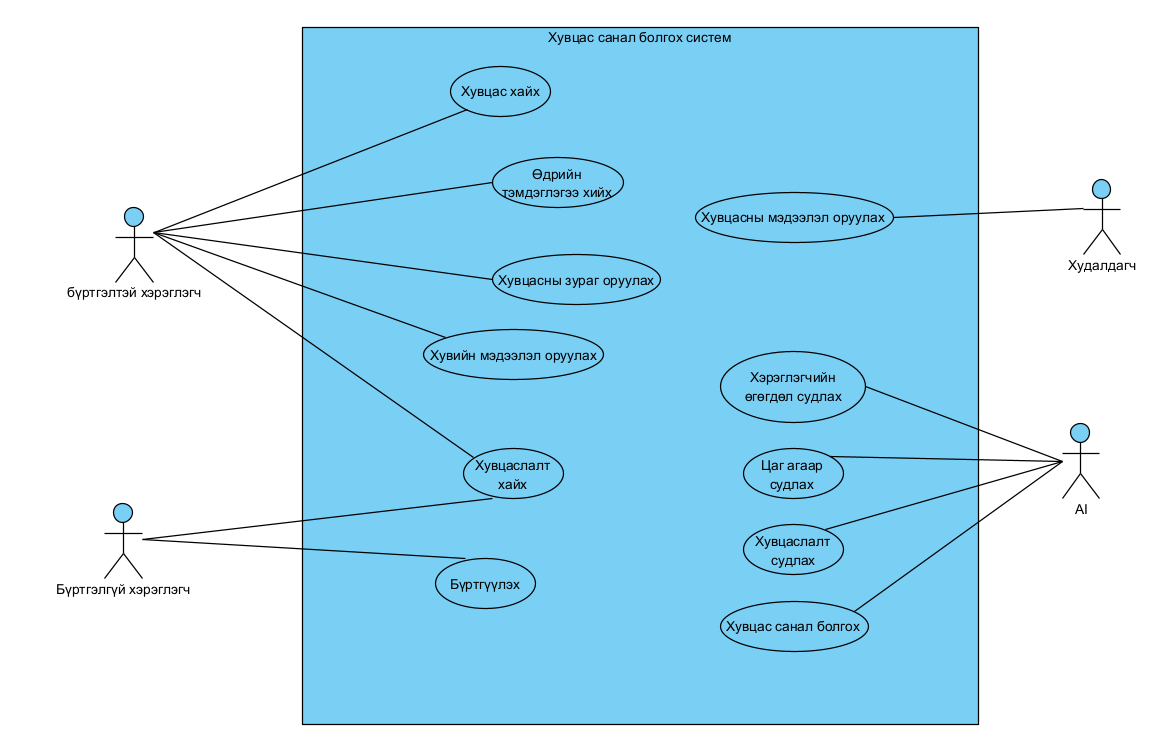
\includegraphics[width=\textwidth]{figures/Usecase.png}
    
    \label{fig:sudalgaa}
\end{figure}
%Visual Paradigm дээр зурсан анхны юзкейс диаграмыг зураг болгон энд оруулна.
%-------------------------------------------------------------------------------

\newpage
\section{Юзкейсийн тодорхойлолт}
\begin{longtable}{|r|p{11.5cm}|}
    \caption{Хувцас санал болгох юзкейсийн тодорхойлолт} 
    \label{table:songolt1}\\ \hline
    {Юзкейс:} & {Хувцас санал болгох}\\ \hline
    {ID:} & {UC01}\\ \hline
    {Үүсгэсэн:} & {Тэмүүлэн}\\ \hline
    {Үүсгэсэн огноо:} & {2024-10-10}\\ \hline
    {Үндсэн тоглогч:} & {Хувцасны сонголт хүссэн хэрэглэгч}\\ \hline
    {Нэмэлт тоглогч:} & {AI систем, Хувцасны өгөгдлийн сан}\\ \hline
    {Товч тайлбар:} & {Хэрэглэгчийн сонголт болон өгөгдсөн өгөгдөл дээр үндэслэн хувцасны сонголтыг санал болгох үйлдэл.}\\ \hline
    {Өмнөх нөхцөл:} & {Хэрэглэгч системд бүртгүүлж, хувийн мэдээллээ оруулсан байна. Хувцасны өгөгдлийн сантай холбогдсон байх.}\\ \hline
    {Үндсэн урсгал:} & {\begin{enumerate}
        \item Хэрэглэгч хувцасны сонголт хийхийг хүсэж байна гэж системд мэдээлнэ.
    \item AI систем нь хэрэглэгчийн өгөгдлийг уншиж, тухайн хүний сонголт болон цаг агаарын мэдээлэл дээр үндэслэн хувцасны сонголт санал болгоно.
    \item Хувцасны сонголтуудыг хэрэглэгчид харуулна.\end{enumerate}}\\\hline
    {Дараах нөхцөл:} & {Хэрэглэгч сонголтод сэтгэл ханамжтай болсноор сонгосон хувцаснуудыг хадгална.}\\ \hline
    {Альтернатив урсгал:} & {\begin{enumerate}
        \itemХэрэв хэрэглэгч системийн санал болгосон хувцаснуудад сэтгэл хангалуун бус байвал AI систем дахин сонголт санал болгоно. 
    \end{enumerate} }\\ \hline
\end{longtable}
\newpage
\begin{longtable}{|r|p{11.5cm}|}
    \caption{Хувцас судлах юзкейсийн тодорхойлолт} 
    \label{table:songolt2}\\ \hline
    {Юзкейс:} & {Хувцаслалт судлах}\\ \hline
    {ID:} & {UC02}\\ \hline
    {Үүсгэсэн:} & {Цогтбаяр}\\ \hline
    {Үүсгэсэн огноо:} & {2024-10-10}\\ \hline
    {Үндсэн тоглогч:} & {AI систем}\\ \hline
    {Нэмэлт тоглогч:} & {Бүртгэлтэй хэрэглэгч}\\ \hline
    {Товч тайлбар:} & {Бүртгэлтэй хэрэглэгчийн байгаа хувцас, хувийн мэдээлэл, хэрэглэгчийн байгаа газрын цаг агаар болон орчин үеийн хувцаслалтын хэв маяг зэргээс хувцаслалт судлах}\\ \hline
    {Өмнөх нөхцөл:} & {\begin{enumerate}
        \item Бүртгэлтэй хэрэглэгч өөрийн хувийн мэдээллийг системд оруулсан байх(Биеийн хэлбэр, жин, нас, хүйс, дуртай өнгө гэх мэт)
        \item Цаг агаарын мэдээлэл судлагдсан байх
        \item Орчин үеийн хувцаслалтуудыг судлах
    \end{enumerate}}\\ \hline
    {Үндсэн урсгал:} & {\begin{enumerate}    
        \item Бүртгэлтэй хэрэглэгчийн оруулсан мэдээлэлд судалгаа хийх
    \item Хэрэглэгчийн байгаа газрын цаг агаарын мэдээлэлд судалгаа хийх
    \item Орчин үеийн хувцаслалтыг хэрэглэгчийн мэдээлэлд тулгуурлсан судалгаа хийх
    \item Хийгдсэн судалгаануудаас нэгтгэж хувцаслалтын шийдлүүдийг гаргаж ирэх.\end{enumerate}}\\ \hline
    {Дараах нөхцөл:} & {Хэрэглэгчид хувцаслалтын шийдлүүдийг гаргаж харуулах}\\ \hline
    {Альтернатив урсгал:} & {\begin{enumerate}
        \item Хэрэглэгчийн мэдээллүүдийг авах
        \item Орчин үеийн хувцаслалтын мэдээллүүдээс шүүлт хийх
    \end{enumerate}}\\ \hline
\end{longtable}
\newpage
\begin{longtable}{|r|p{11.5cm}|}
    \caption{Цаг агаар судлах юзкейсийн тодорхойлолт} 
    \label{table:songolt1}\\ \hline
    {Юзкейс:} & {Цаг агаар судлах}\\ \hline
    {ID:} & {UC03}\\ \hline
    {Үүсгэсэн:} & {Цогтбаяр}\\ \hline
    {Үүсгэсэн огноо:} & {2024-10-10}\\ \hline
    {Үндсэн тоглогч:} & {AI систем}\\ \hline
    {Нэмэлт тоглогч:} & {Бүртгэлтэй хэрэглэгч}\\ \hline
    {Товч тайлбар:} & {Хэрэглэгчийн маргааш эсвэл ирээдүйн хувцас сонголтод зориулж тухайн өдрийн цаг агаарыг судлах}\\ \hline
    {Өмнөх нөхцөл:} & {\begin{enumerate}
        \item Тухайн хэрэглэгчийн байгаа газрын цаг агаар мэдэгдэл гарсан байх
        \item Хэрэглэгч өөрийн location г оруулсан байх 
    \end{enumerate}}\\ \hline
    {Үндсэн урсгал:} & {
    \begin{enumerate}
        \item Хэрэглэгчийн тухайн газрын цаг агаарын мэдэгдэл гарсан байна.
        \item Хэрэглэгчийн байгаа газрын цаг агаарыг тухайн цаг агаарын системээс авна.
       \end{enumerate}}\\ \hline
    {Дараах нөхцөл:} & {Хэрэглэгчийн сонгосон өдөрт зориулсан хувцаслалтыг санал болгох}\\ \hline
    {Альтернатив урсгал:} & {\begin{enumerate}
        \item Хэрэв хэрэглэгчид тухайн өдрийн цаг агаарт тулгуурлан гаргасан хувцаслалт хэрэглэгчид тухайн өдөрт тохирсон байвал хэрэглэгчид үргэлжлүүлэн зөвлөх  
        \item Хэрэглэгчид тухайн хувцас тохироогүй буюу таалагдаагүй байвал хэрэглэгчээс асуумж авч дахин цаг агаарыг болон тухайн цаг агаарт тохирох хувцасыг дахин судална.
        \end{enumerate}}\\ \hline
\end{longtable}
\newpage
\begin{longtable}{|r|p{11.5cm}|}
    \caption{Хэрэглэгчийн өгөгдөл судлах юзкейсийн тодорхойлолт} 
    \label{table:songolt3}\\ \hline
    {Юзкейс:} & {Хэрэглэгчийн өгөгдөл судлах}\\ \hline
    {ID:} & {UC04}\\ \hline
    {Үүсгэсэн:} & {Отгон }\\ \hline
    {Үүсгэсэн огноо:} & {2024-10-10}\\ \hline
    {Үндсэн тоглогч:} & {АI систем эсвэл хэрэглэгчийн өгөгдлийг судлах шинжээч}\\ \hline
    {Нэмэлт тоглогч:} & {Хэрэглэгч, Хэрэглэгчийн өгөгдлийн сан}\\ \hline
    {Товч тайлбар:} & {AI систем эсвэл шинжээч хэрэглэгчийн хувийн болон зан төлөвийн өгөгдлийг судлах, ангилах, шинжлэх үйлдэл.}\\ \hline
    {Өмнөх нөхцөл:} & {Хэрэглэгч системд бүртгүүлсэн, хувийн мэдээлэл бүрэн оруулсан байна. Хэрэглэгчийн зан төлөвийн өгөгдөл цугларсан байна.}\\ \hline
    {Үндсэн урсгал:} & {\begin{enumerate}
        \item Хэрэглэгчийн өгөгдөл судлах хүсэлтийг AI систем эсвэл шинжээчид илгээнэ.
    \item AI систем нь хэрэглэгчийн хувийн болон зан төлөвийн өгөгдлийг шинжилнэ.
    \item Хэрэглэгчийн өгөгдлийн судалгааны үр дүнг харуулна (жишээ нь: хэрэглэгчийн хандлага, хүсэл сонирхол, хэрэглээний загвар).\end{enumerate}}\\ \hline
    {Дараах нөхцөл:} & {Судалгааны үр дүнг өгөгдлийн санд хадгалж, хэрэглэгчийн профайлыг шинэчилсэн байна.}\\ \hline
    {Альтернатив урсгал:} & {1. Хэрэв хэрэглэгчийн өгөгдөл дутуу эсвэл алдаатай бол шинжээч эсвэл AI систем нэмэлт өгөгдөл шаардлага тавина.}\\ \hline
\end{longtable}
\newpage
\begin{longtable}{|r|p{11.5cm}|}
    \caption{Хувцасны мэдээлэл оруулах юзкейсийн тодорхойлолт} 
    \label{table:songolt3}\\ \hline
    {Юзкейс:} & {Хувцасны мэдээлэл оруулах}\\ \hline
    {ID:} & {UC05}\\ \hline
    {Үүсгэсэн:} & {Цогтбаяр}\\ \hline
    {Үүсгэсэн огноо:} & {2024-10-10}\\ \hline
    {Үндсэн тоглогч:} & {Худалдагч}\\ \hline
    {Нэмэлт тоглогч:} & {Хэрэглэгч, AI систем}\\ \hline
    {Товч тайлбар:} & {Худалдагч өөрийн зарж борлуулах хувцасны мэдээллийг зурган болон бичвэр хэлбэрээр оруулах}\\ \hline
    {Өмнөх нөхцөл:} & {\begin{enumerate}
        \item Борлуулах гэж байгаа хувцасныхаа зургийг 4 талаас нь дарах
        \item Хувцасныхаа материал үнэ зэрэг мэдээллүүдийг бэлдэх
    \end{enumerate}}\\ \hline
    {Үндсэн урсгал:} & {\begin{enumerate}
        \item Худалдагч өөрийн борлуулах гэж байгаа хувцасны зурган болон бусад мэдээллүүдийг оруулах
    \item Оруулсан мэдээллийг хэрэглэгчид ойлгомжтой байх эсэхийг шалгах
    \item Шалгагдсан мэдээллийг хэрэглэгчид харах боломжтой болгох.\end{enumerate}}\\ \hline
    {Дараах нөхцөл:} & {Хэрэглэгчид тухайн хувцасны зураг болон бусад мэдээллийг харах}\\ \hline
    {Альтернатив урсгал:} & {\begin{enumerate}
        \item Хэрэглэгчийн хувцаслалтанд дутуу байгаа хувцаснуудыг хэрэглэгчид харуулах
        \item Худалдагчийн оруулсан хувцаснуудаас хэрэглэгчид хэрэгтэй хувцасыг хайн олох
        \item Олсон хувцасыг хэрэглэгчид харуулах
    \end{enumerate}}\\ \hline
\end{longtable}
\newpage
\begin{longtable}{|r|p{11.5cm}|}
    \caption{Хувцас хайх юзкейсийн тодорхойлолт} 
    \label{table:songolt3}\\ \hline
    {Юзкейс:} & {Хувцас хайх}\\ \hline
    {ID:} & {UC06}\\ \hline
    {Үүсгэсэн:} & {Цогтбаяр}\\ \hline
    {Үүсгэсэн огноо:} & {2024-10-10}\\ \hline
    {Үндсэн тоглогч:} & {Бүртгэлтэй хэрэглэгч}\\ \hline
    {Нэмэлт тоглогч:} & {Систем}\\ \hline
    {Товч тайлбар:} & {Хэрэглэгчид хэрэгцээт хувцасыг худалдагчийн оруулсан хувцасны зураг болон мэдээлэл дундаас хайх}\\ \hline
    {Өмнөх нөхцөл:} & {\begin{enumerate}
        \item Хэрэгцээт хувцас хэрэглэгчид гарч ирсэн байх
    \end{enumerate}}\\ \hline
    {Үндсэн урсгал:} & {\begin{enumerate}
        \item Хэрэглэгч нь хайх хэсэг рүү орно.
    \item Өөрт хэрэгцээт хувцасыг хайх
   \end{enumerate}}\\ \hline
    {Дараах нөхцөл:} & {Хэрэглэгч хайсан хувцасаа олох}\\ \hline
    {Альтернатив урсгал:} & {\begin{enumerate}
        \item Хайсан хувцас нь байхгүй байх
    \end{enumerate}}\\ \hline
\end{longtable}
\newpage
\begin{longtable}{|r|p{11.5cm}|}
    \caption{Өдрийн тэмдэглэгээ хийх юзкейсийн тодорхойлолт} 
    \label{table:songolt3}\\ \hline
    {Юзкейс:} & {Өдрийн тэмдэглэгээ хийх}\\ \hline
    {ID:} & {UC07}\\ \hline
    {Үүсгэсэн:} & {Цогтбаяр}\\ \hline
    {Үүсгэсэн огноо:} & {2024-10-10}\\ \hline
    {Үндсэн тоглогч:} & {Бүртгэлтэй хэрэглэгч}\\ \hline
    {Нэмэлт тоглогч:} & {Систем}\\ \hline
    {Товч тайлбар:} & {Хэрэглэгч өөрийн онцгой өдөр болон төлөвлөгөөт өдрүүдийг системийн календар хэсэг тэмдэглэх}\\ \hline
    {Өмнөх нөхцөл:} & {\begin{enumerate}
        \item Хэрэглэгчид тэмдэглэх хэрэгтэй төлөвлөгөөт өдөр байх
    \end{enumerate}}\\ \hline
    {Үндсэн урсгал:} & {\begin{enumerate}
        \item Хэрэглэгч нь календар хэсэг рүү орно.
        \item Календар хэсэгт өөрийн төлөвлөгөөт өдрийг тэмдэглэх
   \end{enumerate}}\\ \hline
    {Дараах нөхцөл:} & {Төлөвлөгөөт өдөрт зориулсан хувцаслалт гаргаж өгөх\\ \hline
    {Альтернатив урсгал:} & {\begin{enumerate}
    \end{enumerate}}\\ \hline
\end{longtable}
\newpage
\begin{longtable}{|r|p{11.5cm}|}
    \caption{Хувцасны зураг оруулах юзкейсийн тодорхойлолт} 
    \label{table:songolt3}\\ \hline
    {Юзкейс:} & {Хувцасны зураг оруулах}\\ \hline
    {ID:} & {UC08}\\ \hline
    {Үүсгэсэн:} & {Цогтбаяр}\\ \hline
    {Үүсгэсэн огноо:} & {2024-10-10}\\ \hline
    {Үндсэн тоглогч:} & {Бүртгэлтэй хэрэглэгч}\\ \hline
    {Нэмэлт тоглогч:} & {Систем}\\ \hline
    {Товч тайлбар:} & {Хэрэглэгч өөрт байгаа  хувцасны зургийг системд оруулах }\\ \hline
    {Өмнөх нөхцөл:} & {\begin{enumerate}
        \item Хувцасны шүүгээнд оруулах гэж байгаа хувцасныхаа зургийг 4 талаас нь дарах
    \end{enumerate}}\\ \hline
    {Үндсэн урсгал:} & {\begin{enumerate}
        \item Хувцасны зургийг системийн шүүгээнд оруулах 
    \item Оруулсан зургийн чанар шалгах
    \item Шалгагдсан зургийг шүүгээнд оруулах\end{enumerate}}\\ \hline
    {Дараах нөхцөл:} & {Хэрэглэгч тухайн хувцасны зургийг шүүгээнээс харах}\\ \hline
    {Альтернатив урсгал:} & {\begin{enumerate}
        \item Чанар муутай хувцасны зурагт сануулга өгөөд дахин зураг дарахыг хүсэх
    \end{enumerate}}\\ \hline
\end{longtable}
\newpage
\begin{longtable}{|r|p{11.5cm}|}
    \caption{Хувийн мэдээлэл оруулах юзкейсийн тодорхойлолт} 
    \label{table:songolt3}\\ \hline
    {Юзкейс:} & {Хувийн мэдээлэл оруулах}\\ \hline
    {ID:} & {UC09}\\ \hline
    {Үүсгэсэн:} & {Цогтбаяр}\\ \hline
    {Үүсгэсэн огноо:} & {2024-10-10}\\ \hline
    {Үндсэн тоглогч:} & {Бүртгэлтэй хэрэглэгч}\\ \hline
    {Нэмэлт тоглогч:} & {Систем}\\ \hline
    {Товч тайлбар:} & {Хэрэглэгч нь өөрийн биеийн жин, биеийн хэлбэр зэрэг хувийн мэдээллүүдийг системд оруулах }\\ \hline
    {Өмнөх нөхцөл:} & {\begin{enumerate}
        \item Өөрийн биеийн өндөр, жин зэргийг үзэх
    \end{enumerate}}\\ \hline
    {Үндсэн урсгал:} & {\begin{enumerate}
        \item Биеийн жин болон биеийн өндөр гэх мэт хувийн мэдээлүүдийг системд оруулах 
    \item Оруулсан мэдээлүүдийг шалгах\end{enumerate}}\\ \hline
    {Дараах нөхцөл:} & {AI систем нь тухайн мэдээллүүдээс судалгаа хийж хэрэглэгчид хувцаслалт санал болгоно.\\ \hline
    {Альтернатив урсгал:} & {\begin{enumerate}
        \item Хэрэглэгчийн оруулсан мэдээлэл нь худал байх үед сануулга илгээх
    \end{enumerate}}\\ \hline
\end{longtable}
\newpage
\begin{longtable}{|r|p{11.5cm}|}
    \caption{Хувцаслалт хайх юзкейсийн тодорхойлолт} 
    \label{table:songolt3}\\ \hline
    {Юзкейс:} & {Хувцаслалт хайх}\\ \hline
    {ID:} & {UC10}\\ \hline
    {Үүсгэсэн:} & {Цогтбаяр}\\ \hline
    {Үүсгэсэн огноо:} & {2024-10-10}\\ \hline
    {Үндсэн тоглогч:} & {Бүртгэлтэй хэрэглэгч, Бүртгэлгүй хэрэглэгч}\\ \hline
    {Нэмэлт тоглогч:} & {Систем}\\ \hline
    {Товч тайлбар:} & {Орчин үеийн хувцаслалтуудыг хайх }\\ \hline
    {Өмнөх нөхцөл:} & {\begin{enumerate}
        \item Өөр өөр төрлийн хувцаслалт сонирхох
    \end{enumerate}}\\ \hline
    {Үндсэн урсгал:} & {\begin{enumerate}
        \item Сонирхсон хувцаслалтуудыг системээс хайх 
        \end{enumerate}}\\ \hline
    {Дараах нөхцөл:} & { Өөрт хэрэгцээт хувцаслалтыг олох }\\ \hline
    {Альтернатив урсгал:} & {\begin{enumerate}
    \end{enumerate}}\\ \hline
\end{longtable}
\newpage
\begin{longtable}{|r|p{11.5cm}|}
    \caption{Бүртгүүлэх юзкейсийн тодорхойлолт} 
    \label{table:songolt3}\\ \hline
    {Юзкейс:} & {Бүртгүүлэх}\\ \hline
    {ID:} & {UC11}\\ \hline
    {Үүсгэсэн:} & {Цогтбаяр}\\ \hline
    {Үүсгэсэн огноо:} & {2024-10-10}\\ \hline
    {Үндсэн тоглогч:} & {Бүртгэлгүй хэрэглэгч}\\ \hline
    {Нэмэлт тоглогч:} & {Систем}\\ \hline
    {Товч тайлбар:} & {Системийн бүрэн гүйцэт ашиглахын тулд бүртгүүлэх}\\ \hline
    {Өмнөх нөхцөл:} & {\begin{enumerate}
        \item Системийн бүртгүүлэх хэсэг рүү орно.
    \end{enumerate}}\\ \hline
    {Үндсэн урсгал:} & {\begin{enumerate}
        \item Системд бүртгүүлэхийн тулд өөрийн нэр, утасны дугаар зэрэг мэдээллүүдийг оруулах
        \item Өөрийн бүртгэлийг баталгаажуулах
        \end{enumerate}}\\ \hline
    {Дараах нөхцөл:} & {Өөрийн гэсэн бүртгэлтэй болох }\\ \hline
    {Альтернатив урсгал:} & {\begin{enumerate}
    \end{enumerate}}\\ \hline
\end{longtable}
%Юзкейсийн тодорхойлолтуудыг бүрэн оруулна.
%-------------------------------------------------------------------------------
\section{Дэвшилтэт юзкейс диаграм}
\begin{figure}[H]
    \centering
    \caption{Системд нэвтэрсэний дараах }
    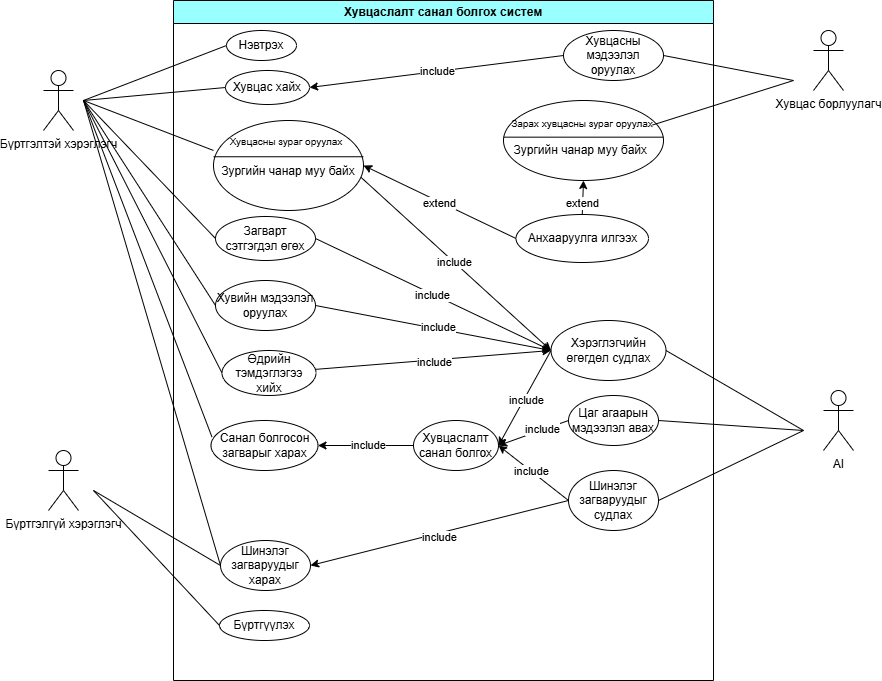
\includegraphics[width=\textwidth]{figures/shaardlagalab7.drawio (1).png}
    
    \label{fig:sudalgaa}
\end{figure}
%Visual Paradigm дээр зурсан дэвшилтэт хэлбэрийн юзкейс диаграмыг зураг болгон энд оруулна.
%-------------------------------------------------------------------------------
\section{Дэвшилтэт юзкейсийн тодорхойлолт}
%Дэвшилтэт юзкейсийн тодорхойлолтуудыг бүрэн оруулна.
\newpage
\begin{longtable}{|r|p{11.5cm}|}
    \caption{Хувцаслалт санал болгох юзкейсийн тодорхойлолт} 
    \label{table:songolt1}\\ \hline
    {Юзкейс:} & {Хувцаслалт санал болгох}\\ \hline
    {ID:} & {UC01}\\ \hline
    {Үүсгэсэн:} & {Тэмүүлэн}\\ \hline
    {Үүсгэсэн огноо:} & {2024-10-10}\\ \hline
    {Үндсэн тоглогч:} & {Хувцасны сонголт хүссэн хэрэглэгч}\\ \hline
    {Нэмэлт тоглогч:} & {AI систем, Хувцасны өгөгдлийн сан}\\ \hline
    {Товч тайлбар:} & {Хэрэглэгчийн сонголт болон өгөгдсөн өгөгдөл дээр үндэслэн хувцасны сонголтыг санал болгох үйлдэл.}\\ \hline
    {Өмнөх нөхцөл:} & {Хэрэглэгч системд бүртгүүлж, хувийн мэдээллээ оруулсан байна. Хувцасны өгөгдлийн сантай холбогдсон байх.}\\ \hline
    {Үндсэн урсгал:} & {\begin{enumerate}
        \item Хэрэглэгч хувцасны сонголт хийхийг хүсэж байна гэж системд мэдээлнэ.
    \item AI систем нь хэрэглэгчийн өгөгдлийг уншиж, тухайн хүний сонголт болон цаг агаарын мэдээлэл дээр үндэслэн хувцасны сонголт санал болгоно.
    \item Хувцасны сонголтуудыг хэрэглэгчид харуулна.\end{enumerate}}\\\hline
    {Дараах нөхцөл:} & {Хэрэглэгч сонголтод сэтгэл ханамжтай болсноор сонгосон хувцаснуудыг хадгална.}\\ \hline
    {Альтернатив урсгал:} & {\begin{enumerate}
        \itemХэрэв хэрэглэгч системийн санал болгосон хувцаснуудад сэтгэл хангалуун бус байвал AI систем дахин сонголт санал болгоно. 
    \end{enumerate} }\\ \hline
        {Include :} & {\begin{enumerate}
        \item Санал болгох загварыг харах юзкейс
    \end{enumerate}}\\ \hline
\end{longtable}
\newpage
\begin{longtable}{|r|p{11.5cm}|}
    \caption{Хувцас судлах юзкейсийн тодорхойлолт} 
    \label{table:songolt2}\\ \hline
    {Юзкейс:} & {Шинэлэг загваруудыг судлах}\\ \hline
    {ID:} & {UC02}\\ \hline
    {Үүсгэсэн:} & {Цогтбаяр}\\ \hline
    {Үүсгэсэн огноо:} & {2024-10-10}\\ \hline
    {Үндсэн тоглогч:} & {AI систем}\\ \hline
    {Нэмэлт тоглогч:} & {Бүртгэлтэй хэрэглэгч}\\ \hline
    {Товч тайлбар:} & {Бүртгэлтэй хэрэглэгчийн байгаа хувцас, хувийн мэдээлэл, хэрэглэгчийн байгаа газрын цаг агаар болон орчин үеийн хувцаслалтын хэв маяг зэргээс хувцаслалт судлах}\\ \hline
    {Өмнөх нөхцөл:} & {\begin{enumerate}
        \item Бүртгэлтэй хэрэглэгч өөрийн хувийн мэдээллийг системд оруулсан байх(Биеийн хэлбэр, жин, нас, хүйс, дуртай өнгө гэх мэт)
        \item Цаг агаарын мэдээлэл судлагдсан байх
        \item Орчин үеийн хувцаслалтуудыг судлах
    \end{enumerate}}\\ \hline
    {Үндсэн урсгал:} & {\begin{enumerate}    
        \item Бүртгэлтэй хэрэглэгчийн оруулсан мэдээлэлд судалгаа хийх
    \item Хэрэглэгчийн байгаа газрын цаг агаарын мэдээлэлд судалгаа хийх
    \item Орчин үеийн хувцаслалтыг хэрэглэгчийн мэдээлэлд тулгуурлсан судалгаа хийх
    \item Хийгдсэн судалгаануудаас нэгтгэж хувцаслалтын шийдлүүдийг гаргаж ирэх.\end{enumerate}}\\ \hline
    {Дараах нөхцөл:} & {Хэрэглэгчид хувцаслалтын шийдлүүдийг гаргаж харуулах}\\ \hline
    {Альтернатив урсгал:} & {\begin{enumerate}
        \item Хэрэглэгчийн мэдээллүүдийг авах
        \item Орчин үеийн хувцаслалтын мэдээллүүдээс шүүлт хийх
    \end{enumerate}}\\ \hline
    {Include :} & {\begin{enumerate}
        \item Шинэлэг загваруудыг харах юзкейс
        \item Хувцаслалт санал болгох
    \end{enumerate}}\\ \hline
\end{longtable}
\begin{longtable}{|r|p{11.5cm}|}
    \caption{Цаг агаар судлах юзкейсийн тодорхойлолт} 
    \label{table:songolt1}\\ \hline
    {Юзкейс:} & {Цаг агаарын мэдээлэл авах}\\ \hline
    {ID:} & {UC03}\\ \hline
    {Үүсгэсэн:} & {Цогтбаяр}\\ \hline
    {Үүсгэсэн огноо:} & {2024-10-10}\\ \hline
    {Үндсэн тоглогч:} & {AI систем}\\ \hline
    {Нэмэлт тоглогч:} & {Бүртгэлтэй хэрэглэгч}\\ \hline
    {Товч тайлбар:} & {Хэрэглэгчийн маргааш эсвэл ирээдүйн хувцас сонголтод зориулж тухайн өдрийн цаг агаарыг судлах}\\ \hline
    {Өмнөх нөхцөл:} & {\begin{enumerate}
        \item Тухайн хэрэглэгчийн байгаа газрын цаг агаар мэдэгдэл гарсан байх
        \item Хэрэглэгч өөрийн location г оруулсан байх 
    \end{enumerate}}\\ \hline
    {Үндсэн урсгал:} & {
    \begin{enumerate}
        \item Хэрэглэгчийн тухайн газрын цаг агаарын мэдэгдэл гарсан байна.
        \item Хэрэглэгчийн байгаа газрын цаг агаарыг тухайн цаг агаарын системээс авна.
       \end{enumerate}}\\ \hline
    {Дараах нөхцөл:} & {Хэрэглэгчийн сонгосон өдөрт зориулсан хувцаслалтыг санал болгох}\\ \hline
    {Альтернатив урсгал:} & {\begin{enumerate}
        \item Хэрэв хэрэглэгчид тухайн өдрийн цаг агаарт тулгуурлан гаргасан хувцаслалт хэрэглэгчид тухайн өдөрт тохирсон байвал хэрэглэгчид үргэлжлүүлэн зөвлөх  
        \item Хэрэглэгчид тухайн хувцас тохироогүй буюу таалагдаагүй байвал хэрэглэгчээс асуумж авч дахин цаг агаарыг болон тухайн цаг агаарт тохирох хувцасыг дахин судална.
        \end{enumerate}}\\ \hline
        {Include :} & {\begin{enumerate}
        \item Хувцаслалт санал болгох юзкейс
    \end{enumerate}}\\ \hline
\end{longtable}
\newpage
\begin{longtable}{|r|p{11.5cm}|}
    \caption{Хэрэглэгчийн өгөгдөл судлах юзкейсийн тодорхойлолт} 
    \label{table:songolt3}\\ \hline
    {Юзкейс:} & {Хэрэглэгчийн өгөгдөл судлах}\\ \hline
    {ID:} & {UC04}\\ \hline
    {Үүсгэсэн:} & {Отгон }\\ \hline
    {Үүсгэсэн огноо:} & {2024-10-10}\\ \hline
    {Үндсэн тоглогч:} & {АI систем }\\ \hline
    {Нэмэлт тоглогч:} & {Хэрэглэгч, Хэрэглэгчийн өгөгдлийн сан}\\ \hline
    {Товч тайлбар:} & {AI систем хувийн болон зан төлөвийн өгөгдлийг судлах, ангилах, шинжлэх үйлдэл.}\\ \hline
    {Өмнөх нөхцөл:} & {Хэрэглэгч системд бүртгүүлсэн, хувийн мэдээлэл бүрэн оруулсан байна. Хэрэглэгчийн зан төлөвийн өгөгдөл цугларсан байна.}\\ \hline
    {Үндсэн урсгал:} & {\begin{enumerate}
        \item Хэрэглэгчийн өгөгдөл судлах хүсэлтийг AI систем  илгээнэ.
    \item AI систем нь хэрэглэгчийн хувийн болон зан төлөвийн өгөгдлийг шинжилнэ.
    \item Хэрэглэгчийн өгөгдлийн судалгааны үр дүнг харуулна (жишээ нь: хэрэглэгчийн хандлага, хүсэл сонирхол, хэрэглээний загвар).\end{enumerate}}\\ \hline
    {Дараах нөхцөл:} & {Судалгааны үр дүнг өгөгдлийн санд хадгалж, хэрэглэгчийн профайлыг шинэчилсэн байна.}\\ \hline
    {Альтернатив урсгал:} & {1. Хэрэв хэрэглэгчийн өгөгдөл дутуу эсвэл алдаатай байвал AI систем нэмэлт өгөгдөл шаардлага тавина.}\\ \hline
    {Include :} & {\begin{enumerate}
        \item Хувцаслалт санал болгох юзкейс
    \end{enumerate}}\\ \hline
\end{longtable}
\newpage
\begin{longtable}{|r|p{11.5cm}|}
    \caption{Хувцасны мэдээлэл оруулах юзкейсийн тодорхойлолт} 
    \label{table:songolt3}\\ \hline
    {Юзкейс:} & {Хувцасны мэдээлэл оруулах}\\ \hline
    {ID:} & {UC05}\\ \hline
    {Үүсгэсэн:} & {Цогтбаяр}\\ \hline
    {Үүсгэсэн огноо:} & {2024-10-10}\\ \hline
    {Үндсэн тоглогч:} & {Худалдагч}\\ \hline
    {Нэмэлт тоглогч:} & {Хэрэглэгч, AI систем}\\ \hline
    {Товч тайлбар:} & {Худалдагч өөрийн зарж борлуулах хувцасны мэдээллийг бичвэр хэлбэрээр оруулах}\\ \hline
    {Өмнөх нөхцөл:} & {\begin{enumerate}
        \item Хувцасныхаа материал үнэ зэрэг мэдээллүүдийг бэлдэх
    \end{enumerate}}\\ \hline
    {Үндсэн урсгал:} & {\begin{enumerate}
        \item Худалдагч өөрийн борлуулах гэж байгаа хувцасны зурган болон бусад мэдээллүүдийг оруулах
    \item Оруулсан мэдээллийг хэрэглэгчид ойлгомжтой байх эсэхийг шалгах
    \item Шалгагдсан мэдээллийг хэрэглэгчид харах боломжтой болгох.\end{enumerate}}\\ \hline
    {Дараах нөхцөл:} & {Хэрэглэгчид тухайн хувцасны зураг болон бусад мэдээллийг харах}\\ \hline
    {Альтернатив урсгал:} & {\begin{enumerate}
        \item Хэрэглэгчийн хувцаслалтанд дутуу байгаа хувцаснуудыг хэрэглэгчид харуулах
        \item Худалдагчийн оруулсан хувцаснуудаас хэрэглэгчид хэрэгтэй хувцасыг хайн олох
        \item Олсон хувцасыг хэрэглэгчид харуулах
    \end{enumerate}}\\ \hline
     {Include :} & {\begin{enumerate}
        \item Хувцаслалт хайх юзкейс
    \end{enumerate}}\\ \hline
\end{longtable}
\newpage
\begin{longtable}{|r|p{11.5cm}|}
    \caption{Зарах хувцасны зураг оруулах юзкейсийн тодорхойлолт} 
    \label{table:songolt4}\\ \hline
    {Юзкейс:} & {Зарах хувцасны зураг оруулах}\\ \hline
    {ID:} & {UC06}\\ \hline
    {Үүсгэсэн:} & {Цогтбаяр}\\ \hline
    {Үүсгэсэн огноо:} & {2024-10-10}\\ \hline
    {Үндсэн тоглогч:} & {Хувцасны зургийг оруулж буй худалдагч}\\ \hline
    {Нэмэлт тоглогч:} & {Бүртгэлтэй хэрэглэгч}\\ \hline
    {Товч тайлбар:} & {Худалдагч өөрийн борлуулах гэж байгаа хувцасны зургийг манай системд оруулах}\\ \hline
    {Өмнөх нөхцөл:} & {Худалдагч өөрийн борлуулах гэж байгаа хувцасыг 4 талаас нь зургийн чанар сайтайгаар дарна.}\\ \hline
    {Үндсэн урсгал:} & {\begin{enumerate}
        \item Худалдагч дарсан зургийг системд оруулах
        \item Оруулсан зургийг AI хянах
        \item Зургийг хүлээж авах
        \end{enumerate}}\\ \hline
    {Дараах нөхцөл:} & {Дарж оруулсан зургийг хэрэглэгч системээр дамжуулан харах.}\\ \hline
    {Альтернатив урсгал:} & {1.Хэрэв хувцасны зураг чанар муутай байвал хувцасны зургийг дахин дарахыг анхааруулсан анхааруулга илгээх}\\ \hline
     {Extends :} & {\begin{enumerate}
        \item Анхааруулга илгээх юзкейс
    \end{enumerate}}\\ \hline
\end{longtable}
\newpage
\begin{longtable}{|r|p{11.5cm}|}
    \caption{Нэвтрэх юзкейсийн тодорхойлолт} 
    \label{table:songolt4}\\ \hline
    {Юзкейс:} & {Нэвтрэх}\\ \hline
    {ID:} & {UC07}\\ \hline
    {Үүсгэсэн:} & {Цогтбаяр}\\ \hline
    {Үүсгэсэн огноо:} & {2024-10-10}\\ \hline
    {Үндсэн тоглогч:} & {Бүртгэлтэй хэрэглэгч}\\ \hline
    {Нэмэлт тоглогч:} & {Систем}\\ \hline
    {Товч тайлбар:} & {Хэрэглэгч системийг бүрэн ашиглахын тулд нэвтрэх хэрэгтэй.}\\ \hline
    {Өмнөх нөхцөл:} & {Хэрэглэгч нь системд бүртгүүлсэн байх}\\ \hline
    {Үндсэн урсгал:} & {\begin{enumerate}
        \item Хэрэглэгч нэвтрэх хэсэг рүү орох
    \item Хэрэглэгч өөрийн нэвтрэх нэр болон нууц дугаарыг оруулсанаар системд нэвтэрнэ.
    \item Хувцасны мэдээллийг өгөгдлийн санд хадгална.\end{enumerate}}\\ \hline
    {Дараах нөхцөл:} & {Хэрэглэгч системийг ашиглах боломжтой болно.}\\ \hline
    {Альтернатив урсгал:} & {1. Хэрэв хэрэглэгчийн нууц үг болон нэвтрэх нэр нь буруу байвал хэрэглэгчид анхааруулж хэрэглэгч дахин нэвтрэхийг оролдох}\\ \hline
\end{longtable}
\newpage
\begin{longtable}{|r|p{11.5cm}|}
    \caption{Хувцас хайх юзкейсийн тодорхойлолт} 
    \label{table:songolt4}\\ \hline
    {Юзкейс:} & {Хувцас хайх}\\ \hline
    {ID:} & {UC08}\\ \hline
    {Үүсгэсэн:} & {Цогтбаяр}\\ \hline
    {Үүсгэсэн огноо:} & {2024-10-10}\\ \hline
    {Үндсэн тоглогч:} & {Бүртгэлтэй хэрэглэгч}\\ \hline
    {Нэмэлт тоглогч:} & {Худалдагч}\\ \hline
    {Товч тайлбар:} & {Хэрэглэгч өөрт нь хэрэг болох хувцасыг системд оруулсан хувцасны мэдээллүүдээс хайх}\\ \hline
    {Өмнөх нөхцөл:} & {Хэрэглэгч нь системд нэвтэрсэн байх}\\ \hline
    {Үндсэн урсгал:} & {\begin{enumerate}
        \item Системээс санал болгосон хувцаслалт юмуу өөрт таалагдсан хувцаслалтыг харах
    \item Ижил төстэй хувцаслалтыг хайх
    \end{enumerate}}\\ \hline
    {Дараах нөхцөл:} & {Хэрэглэгч өөрт хэрэгтэй хувцасыг олох}\\ \hline
    {Альтернатив урсгал:} & {1. Хэрэглэгчид хэрэгтэй хувцас олдохгүй байх 
    2. Өөр хувцас хайх}\\ \hline
\end{longtable}
\newpage
\begin{longtable}{|r|p{11.5cm}|}
    \caption{Хувцасны зураг оруулах юзкейсийн тодорхойлолт} 
    \label{table:songolt4}\\ \hline
    {Юзкейс:} & {Хувцасны зураг оруулах}\\ \hline
    {ID:} & {UC09}\\ \hline
    {Үүсгэсэн:} & {Цогтбаяр}\\ \hline
    {Үүсгэсэн огноо:} & {2024-10-10}\\ \hline
    {Үндсэн тоглогч:} & {Бүртгэлтэй хэрэглэгч}\\ \hline
    {Нэмэлт тоглогч:} & {AI Систем}\\ \hline
    {Товч тайлбар:} & {Хэрэглэгч өөрийн хувцасны зургийг системийн шүүгээнд оруулах}\\ \hline
    {Өмнөх нөхцөл:} & {Хэрэглэгч нь системд нэвтэрсэн байх}\\ \hline
    {Үндсэн урсгал:} & {\begin{enumerate}
        \item Хэрэглэгч нь өөрийн хувцасны зургийг 4 талаас нь авсан чанар сайтай зургийг оруулах
    \item Хэрэглэгчийн оруулсан зургийг AI систем шалгах
    \item Хувцасны мэдээллийг өгөгдлийн санд хадгална.\end{enumerate}}\\ \hline
    {Дараах нөхцөл:} & {Хэрэглэгчийн шүүгээнд хувцас нь нэмэгдэх}\\ \hline
    {Альтернатив урсгал:} & {1. Хувцасны зургийг чанар муутай илгээсэн тохиолдолд анхааруулга илгээх}\\ \hline
     {Include :} & {\begin{enumerate}
        \item Хэрэглэгчийн өгөгдөл судлах юзкейс
    \end{enumerate}}\\ \hline
     {Extend :} & {\begin{enumerate}
        \item Анхааруулга илгээх юзкейс
    \end{enumerate}}\\ \hline
\end{longtable}
\newpage
\begin{longtable}{|r|p{11.5cm}|}
    \caption{Загварт сэтгэгдэл өгөх юзкейсийн тодорхойлолт} 
    \label{table:songolt4}\\ \hline
    {Юзкейс:} & {Загварт сэтгэгдэл өгөх}\\ \hline
    {ID:} & {UC10}\\ \hline
    {Үүсгэсэн:} & {Цогтбаяр}\\ \hline
    {Үүсгэсэн огноо:} & {2024-10-10}\\ \hline
    {Үндсэн тоглогч:} & {Бүртгэлтэй хэрэглэгч}\\ \hline
    {Нэмэлт тоглогч:} & {AI}\\ \hline
    {Товч тайлбар:} & {Хэрэглэгч нь системийн өөрт нь зориулж гаргасан хувцаслалтанд үнэлгээ өгөх.}\\ \hline
    {Өмнөх нөхцөл:} & {Хэрэглэгчид AI хувцаслалт санал болгосон байх}\\ \hline
    {Үндсэн урсгал:} & {\begin{enumerate}
        \item AI ын санал болгосон хувцаслалтанд сэтгэгдэл өгөх
    \end{enumerate}}\\ \hline
    {Дараах нөхцөл:} & {Хэрэглэгчид тохирох хувцаслалтын сэтгэгдлээс өгөгдөл цуглуулах} \hline
    {Альтернатив урсгал:} & {1. Хэрэглэгчид санал болгосон хувцаслалт байхгүй бол бусад хэрэглэгчидийн хувцаслалтанд сэтгэгдэл үлдээх}\\ \hline
     {Include :} & {\begin{enumerate}
        \item Хэрэглэгчийн өгөгдөл судлах юзкейс
    \end{enumerate}}\\ \hline
\end{longtable}
\newpage
\begin{longtable}{|r|p{11.5cm}|}
    \caption{Өдрийн тэмдэглэгээ хийх юзкейсийн тодорхойлолт} 
    \label{table:songolt4}\\ \hline
    {Юзкейс:} & {Өдрийн тэмдэглэгээ хийх}\\ \hline
    {ID:} & {UC11}\\ \hline
    {Үүсгэсэн:} & {Цогтбаяр}\\ \hline
    {Үүсгэсэн огноо:} & {2024-10-10}\\ \hline
    {Үндсэн тоглогч:} & {Бүртгэлтэй хэрэглэгч}\\ \hline
    {Нэмэлт тоглогч:} & {AI}\\ \hline
    {Товч тайлбар:} & {Хэрэглэгч нь баярын болон өөрт онцгой өдрийг систем дээр тэмдэглэгээ хийх ингэснээр хэрэглэгчид тухайн өдөрт зориулсан хувцаслалтыг санал болгоно. }\\ \hline
    {Өмнөх нөхцөл:} & {Хэрэглэгч системд нэвтэрсэн байх}\\ \hline
    {Үндсэн урсгал:} & {\begin{enumerate}
        \item Өөрийн чухал төлөвлөгөөтэй өдрүүдийг тэмдэглэх
    \end{enumerate}}\\ \hline
    {Дараах нөхцөл:} & {AI нь тэмдэглэсэн өдрийг хүлээн авч тухайн өдөрт зориулсан хувцаслалтыг харуулна.} \hline
    {Альтернатив урсгал:} & { }\\ \hline
     {Include :} & {\begin{enumerate}
        \item Хэрэглэгчийн өгөгдөл судлах юзкейс
    \end{enumerate}}\\ \hline
\end{longtable}
\newpage
\begin{longtable}{|r|p{11.5cm}|}
    \caption{Санал болгосон загварыг харах юзкейсийн тодорхойлолт} 
    \label{table:songolt4}\\ \hline
    {Юзкейс:} & {Санал болгосон загварын харах}\\ \hline
    {ID:} & {UC12}\\ \hline
    {Үүсгэсэн:} & {Цогтбаяр}\\ \hline
    {Үүсгэсэн огноо:} & {2024-10-10}\\ \hline
    {Үндсэн тоглогч:} & {Бүртгэлтэй хэрэглэгч}\\ \hline
    {Нэмэлт тоглогч:} & {AI}\\ \hline
    {Товч тайлбар:} & {Хэрэглэгчийн өгөгдөл болон бусад өгөгдлүүд дээр тулгуурлан гаргасан хувцаслалтыг харах }\\ \hline
    {Өмнөх нөхцөл:} & {Хэрэглэгч системд өөрийн өгөгдлийг өгсөн байх}\\ \hline
    {Үндсэн урсгал:} & {\begin{enumerate}
        \item Хэрэглэгчийн оруулсан өгөгдөлд тулгуурлан хувцаслалт гаргах
        \item Гаргасан хувцаслалтыг харах
    \end{enumerate}}\\ \hline
    {Дараах нөхцөл:} & {Гаргасан хувцаслалт таалагдсан бол туршиж үзнэ.} \hline
    {Альтернатив урсгал:} & {Гаргасан хувцаслалт таалагдаагүй байвал сэтгэгдэл үлдээж дахин хувцаслалт санал болгохыг хүлээх}\\ \hline
\end{longtable}
\newpage
\begin{longtable}{|r|p{11.5cm}|}
    \caption{Шинэлэг загваруудыг харах юзкейсийн тодорхойлолт} 
    \label{table:songolt4}\\ \hline
    {Юзкейс:} & {Шинэлэг загваруудыг харах}\\ \hline
    {ID:} & {UC13}\\ \hline
    {Үүсгэсэн:} & {Цогтбаяр}\\ \hline
    {Үүсгэсэн огноо:} & {2024-10-10}\\ \hline
    {Үндсэн тоглогч:} & {Бүртгэлгүй хэрэглэгч, Бүртгэлтэй хэрэглэгч}\\ \hline
    {Нэмэлт тоглогч:} & {AI}\\ \hline
    {Товч тайлбар:} & {АI ын гаргаж өгсөн шинэлэг хувцаслалтын загваруудыг харах }\\ \hline
    {Өмнөх нөхцөл:} & {Манай системийг ашиглах}\\ \hline
    {Үндсэн урсгал:} & {\begin{enumerate}
        \item АI аас гаргаж өгсөн шинэлэг загваруудыг харах
    \end{enumerate}}\\ \hline
    {Дараах нөхцөл:} & {Гаргасан хувцаслалт таалагдсан бол туршиж үзнэ.} \hline
    {Альтернатив урсгал:} & {Бүртгэлтэй хэрэглэгч гаргасан хувцаслалт таалагдаагүй байвал сэтгэгдэл үлдээж болно.}\\ \hline
\end{longtable}
\newpage
\begin{longtable}{|r|p{11.5cm}|}
    \caption{ Бүртгүүлэх юзкейсийн тодорхойлолт} 
    \label{table:songolt4}\\ \hline
    {Юзкейс:} & {Бүртгүүлэх}\\ \hline
    {ID:} & {UC14}\\ \hline
    {Үүсгэсэн:} & {Цогтбаяр}\\ \hline
    {Үүсгэсэн огноо:} & {2024-10-10}\\ \hline
    {Үндсэн тоглогч:} & {Бүртгэлтэй хэрэглэгч}\\ \hline
    {Нэмэлт тоглогч:} & {Систем}\\ \hline
    {Товч тайлбар:} & {Системд ашиглахад зориулсан бүртгэл үүсгэх}\\ \hline
    {Өмнөх нөхцөл:} & {Системээс өгч буй заавруудыг сайн уншиж өөрийн мэдээллийг системд өгөх\\ \hline
    {Үндсэн урсгал:} & {\begin{enumerate}
        \item Өгсөн мэдээллүүдийг баталгаажуулж судалгаа авах
        \item Нэвтрэх нэр , Нууц үг зэргийг зохиож оруулах
    \end{enumerate}}\\ \hline
    {Дараах нөхцөл:} & {Систем нь өгсөн мэдээллийг баталгаажуулж бүртгэл олгох} \hline
    {Альтернатив урсгал:} & {Өгсөн мэдээллүүд буруу байвал бүртгэл үүсгэж буй хэрэглэгчид сануулга өгөх}\\ \hline
\end{longtable}
\newpage
\begin{longtable}{|r|p{11.5cm}|}
	%\centering
    \caption{Хувцаслалт санал болгох юзкейсийн хэрэглэгч системийн санал болгосон хувцаснуу-
дад сэтгэл хангалуун бус байвал AI систем дахин сон-
голт санал болгох альтернатив урсгал} 
	% цэгийн оронд аль юзкейсийн альтернатив урсгалын нэрийг бичих!!!
	\label{table:alt}\\ \hline
	% alt -н оронд аль юзкейсийн альтернатив урсгал болохыг товчоор Англиар нэрлэх!!!
	
	{Альтернатив урсгалын нэр:} & {Хэрэв хэрэглэгч системийн санал болгосон хувцаснуу-
дад сэтгэл хангалуун бус байвал AI систем дахин сон-
голт санал болгоно.}\\ \hline
	{ID:} & {AUC01}\\ \hline
	{Үүсгэсэн:} & {Цогтбаяр}\\ \hline
	{Үүсгэсэн огноо:} & {2024.10.10}\\ \hline
	{Үндсэн тоглогч:} & {АI}\\ \hline
	{Нэмэлт тоглогч:} & {бүртгэлтэй хэрэглэгч}\\ \hline
	{Товч тайлбар:} & {Хэрэглэгчид зориулж гаргасан хувцаслалт хэрэглэгчид таалагдахгүй байвал дахин хувцаслалтын загвар гаргах }\\ \hline
	{Өмнөх нөхцөл:} & {Хэрэглэгчид хувцас таалагдаагүй байх}\\ \hline
	{Альтернатив урсгал:} & {Хэрэглэгчид зориулж дахин хувцаслалт гаргаж өгөх}\\ \hline
	{Дараах нөхцөл:} & {Хувцаслалтанд хэрэглэгч сэтгэгдэл өгөх}\\ \hline
\end{longtable}  
\newpage
\begin{longtable}{|r|p{11.5cm}|}
	%\centering
    \caption{Хэрэглэгчийн өгөгдөл судлах юзкейсийн хэрэглэгчийн өгөгдөл дутуу эсвэл алдаатай байвал
AI систем нэмэлт өгөгдөл шаардлага тавина. альтернатив урсгал} 
	% цэгийн оронд аль юзкейсийн альтернатив урсгалын нэрийг бичих!!!
	\label{table:alt}\\ \hline
	% alt -н оронд аль юзкейсийн альтернатив урсгал болохыг товчоор Англиар нэрлэх!!!
	
	{Альтернатив урсгалын нэр:} & {Хэрэв хэрэглэгчийн өгөгдөл дутуу эсвэл алдаатай байвал
AI систем нэмэлт өгөгдөл шаардлага тавих}\\ \hline
	{ID:} & {AUC02}\\ \hline
	{Үүсгэсэн:} & {Цогтбаяр}\\ \hline
	{Үүсгэсэн огноо:} & {2024.10.10}\\ \hline
	{Үндсэн тоглогч:} & {АI}\\ \hline
	{Нэмэлт тоглогч:} & {бүртгэлтэй хэрэглэгч}\\ \hline
	{Товч тайлбар:} & {Хэрэглэгчид зориулсан хувцаслалт гаргах боломжгүй байвал дахин нэмж өгөгдөл оруулах шаардлага тавих}\\ \hline
	{Өмнөх нөхцөл:} & {Хэрэглэгчийн өгөгдөл хувцаслалт гаргахад дутмаг байх} \hline
	{Альтернатив урсгал:} & {Хэрэглэгчид шаардлага тавьж нэмж өгөгдөл авах}\\ \hline
	{Дараах нөхцөл:} & {Хэрэглэгчид тохирсон хувцаслалт гаргах}\\ \hline
\end{longtable} 
\newpage
\begin{longtable}{|r|p{11.5cm}|}
	%\centering
    \caption{Зарах хувцасны зураг оруулах юзкейсийн хувцасны зураг чанар муутай байвал хувцасны зур-
гийг дахин дарахыг анхааруулсан анхааруулга илгээх альтернатив урсгал} 
	% цэгийн оронд аль юзкейсийн альтернатив урсгалын нэрийг бичих!!!
	\label{table:alt}\\ \hline
	% alt -н оронд аль юзкейсийн альтернатив урсгал болохыг товчоор Англиар нэрлэх!!!
	
	{Альтернатив урсгалын нэр:} & {хувцасны зураг чанар муутай байвал хувцасны зур-
гийг дахин дарахыг анхааруулсан анхааруулга илгээх}\\ \hline
	{ID:} & {AUC03}\\ \hline
	{Үүсгэсэн:} & {Цогтбаяр}\\ \hline
	{Үүсгэсэн огноо:} & {2024.10.10}\\ \hline
	{Үндсэн тоглогч:} & {Систем}\\ \hline
	{Нэмэлт тоглогч:} & {Хувцасны зургийг оруулж буй худалдагч}\\ \hline
	{Товч тайлбар:} & {Хвцасны зураг чанар муутай байвал хувцасны зур-
гийг дахин дарахыг анхааруулсан анхааруулгыг хувцасныхаа зургийг оруулсан худалдагчид илгээх}\\ \hline
	{Өмнөх нөхцөл:} & {Чанар муутай зураг худалдагч оруулсан байх} \hline
	{Альтернатив урсгал:} & {Зургийн чанарыг сайжруулах хэрэгтэй гэсэн анхааруулгыг илгээх}\\ \hline
	{Дараах нөхцөл:} & {Худалдагч анхууруулгыг авах}\\ \hline
\end{longtable} 
\newpage
\begin{longtable}{|r|p{11.5cm}|}
	%\centering
    \caption{Нэвтрэх юзкейсийн хэрэглэгчийн нууц үг болон нэвтрэх нэр нь буруу
байвал хэрэглэгчид анхааруулж хэрэглэгч дахин нэвтрэхийг
оролдох альтернатив урсгал} 
	% цэгийн оронд аль юзкейсийн альтернатив урсгалын нэрийг бичих!!!
	\label{table:alt}\\ \hline
	% alt -н оронд аль юзкейсийн альтернатив урсгал болохыг товчоор Англиар нэрлэх!!!
	
	{Альтернатив урсгалын нэр:} & {хэрэглэгчийн нууц үг болон нэвтрэх нэр нь буруу
байвал хэрэглэгчид анхааруулж хэрэглэгч дахин нэвтрэхийг
оролдох}\\ \hline
	{ID:} & {AUC04}\\ \hline
	{Үүсгэсэн:} & {Цогтбаяр}\\ \hline
	{Үүсгэсэн огноо:} & {2024.10.10}\\ \hline
	{Үндсэн тоглогч:} & {Систем}\\ \hline
	{Нэмэлт тоглогч:} & {Бүртгэлтэй хэрэглэгч}\\ \hline
	{Товч тайлбар:} & {Нэвтрэх нэр , нууц үгийг буруу оруулсан байвал анхааруулж хэрэглэгчийг дахин нэвтрүүлэх }\\ \hline
	{Өмнөх нөхцөл:} & {Нэвтрэх нэр , нууц үгийг буруу оруулсан байх} \hline
	{Альтернатив урсгал:} & {хэрэглэгчийн нууц үг болон нэвтрэх нэр нь буруу
байвал хэрэглэгчид анхааруулж хэрэглэгчийг дахин нэвтрэхийг
зөвлөх}\\ \hline
	{Дараах нөхцөл:} & {Хэрэглэгч дахин нэвтрэх}\\ \hline
\end{longtable}
\newpage
\begin{longtable}{|r|p{11.5cm}|}
	%\centering
    \caption{Хувцасны зураг оруулах юзкейсийн хувцасны зургийг чанар муутай илгээсэн тохиолдолд ан-
хааруулга илгээх альтернатив урсгал} 
	% цэгийн оронд аль юзкейсийн альтернатив урсгалын нэрийг бичих!!!
	\label{table:alt}\\ \hline
	% alt -н оронд аль юзкейсийн альтернатив урсгал болохыг товчоор Англиар нэрлэх!!!
	
	{Альтернатив урсгалын нэр:} & {Хувцасны зургийг чанар муутай илгээсэн тохиолдолд ан-
хааруулга илгээх}\\ \hline
	{ID:} & {AUC05}\\ \hline
	{Үүсгэсэн:} & {Цогтбаяр}\\ \hline
	{Үүсгэсэн огноо:} & {2024.10.10}\\ \hline
	{Үндсэн тоглогч:} & {Систем}\\ \hline
	{Нэмэлт тоглогч:} & {Бүртгэлтэй хэрэглэгч}\\ \hline
	{Товч тайлбар:} & {Шүүгээнд оруулах гэж байгаа зургийн чанар муу байсан тул систем хэрэглэгч рүү анхааруулга илгээх}\\ \hline
	{Өмнөх нөхцөл:} & {Хэрэглэгч чанар муутай зураг оруулсан байх} \hline
	{Альтернатив урсгал:} & {хувцасны зургийг чанар муутай илгээсэн тул ан-
хааруулга илгээх}\\ \hline
	{Дараах нөхцөл:} & {Хэрэглэгч дахин зураг оруулах}\\ \hline
\end{longtable}
%---------------\section{Системийн үйл ажиллагааны тайлбар}
\section{Шинжилгээний класс}
\subsection{Нэр, үйл үгийн шинжилгээ}

\par

\noindent\textcolor{red}{Бүртгэлгүй хэрэглэгч нь бүртгэл} \textcolor{blue}{үүсгэж} байж системийг бүрэн \textcolor{blue}{ашиглах} боломжтой болно. \textcolor{red}{Бүртгэл} \textcolor{blue}{үүсгэхдээ} \textcolor{red}{өөрийн биеийн хэлбэр, жин, өндөр болон нас, хүйс зэрэг хувийн мэдээллийг системд оруулах}ёстой. Мөн системийн\textcolor{red}{ нэвтрэх нэр болон нууц үгийг} \textcolor{blue}{зохиох} \textcolor{red}{хэрэгтэй ба өөрийн бүртгэлийг утасны дугаар эсвэл mail хаягаар баталгаажуулах} \textcolor{blue}{хэрэгтэй.} \textcolor{red}{Бүртгэлтэй болсон хэрэглэгч} \textcolor{blue}{нь системд өөрийн нууц үг болон нэвтрэх нэрийг оруулан нэвтэрнэ.} \textcolor{red}{Хэрэглэгч өөрийн хувцасны зургийг} \textcolor{blue}{оруулан} \textcolor{red}{системийн хувцасны шүүгээнд нэмж болно.} \textcolor{red}{Хэрэглэгч шүүгээн доторх хувцас} \textcolor{blue}{нэмэх, хасах} \textcolor{red}{үйлдлүүдийг хийж болно.} \textcolor{red}{Хэрэглэгч нь мөн өөрийн шүүгээнд буй хувцлын тэмдэглэсэн өдөр, төлөвлөгөөт өдөр зэргийг оруулснаар тухайн өдөр өмсөх хувцасны загварыг цаг агаарын мэдээлэл болон одоо шүүгээнд байгаа хувцсанд мөн хэрэглэгчийн хувийн мэдээлэлд хиймэл оюун ухаанаар} \textcolor{blue}{дүн шинжилгээ хийлгэсний} \textcolor{red}{дараагаар хэрэглэгчид тохирох хувцаслалтуудыг} \textcolor{blue}{зохиох} \textcolor{red}{хэрэглэгчид санал болгоно.} \textcolor{red}{Санал болгосон загваруудаас хэрэглэгч өөрийн} \textcolor{blue}{таалагдсан загварыг} \textcolor{red}{өөрийн загварын цуглуулганд} \textcolor{blue}{нэмж болно.} \textcolor{red}{Загварыг өөрчлөх} \textcolor{blue}{засаж хадгалах} \textcolor{red}{боломжтой.} \textcolor{red}{Мөн хувцаслалтад дутсан хувцаснуудаас системийн зүгээс санал болгож} \textcolor{blue}{хувцасыг худалдан авах хэрэглэгчийг холбож өгөх} \textcolor{red}{болно.} \textcolor{red}{Зөвхөн дутсан хувцсыг хэрэглэгч нь худалдан авч} \textcolor{blue}{сонирхох, хайж} \textcolor{red}{боломжтой.} \textcolor{red}{Эдгээрийг бүртгэл} \textcolor{blue}{үүсгэсний} \textcolor{red}{дараа хийж болох бөгөөд бүртгэлтэй хэрэглэгчид мэдээлэл дутмаг үед} \textcolor{red}{хэрэглэгч өөрийн хувийн мэдээллүүдийг} \textcolor{blue}{бүртгэлтэй хэрэглэгчийн бүртгэлд болон бүртгэлтэй} \textcolor{red}{хэрэглэгчид хадгалах боломжтой.} \textcolor{blue}{Бүртгэлтэй хэрэглэгч} \textcolor{red}{нь мөн өөрийн} \textcolor{blue}{борлуулсан хувцас} \textcolor{red}{буюу өөрийн хувцасны мэдээллийг манай онлайн дэлгүүрт тавьснаар хэрэглэгчид} \textcolor{blue}{хүргэх} \textcolor{red}{боломжтой болно.} \textcolor{red}{Худалдагч болон бүртгэлтэй хэрэглэгч нь хувцасаа зурганд хэлбэрээр оруулах хэрэгтэй.}




\subsection{Бүртгэлгүй хэрэглэгч}
Бүртгэлгүй хэрэглэгч нь системд бүртгэл үүсгээгүй, хязгаарлагдмал үйлдэл хийх боломжтой. Бүртгэл үүсгэснээр дараах боломжуудыг олж авна:
\begin{itemize}
    \item Системд нэвтрэх
    \item Хувийн мэдээлэл оруулах
    \item Хувцасны зураг оруулж, шүүгээнд нэмэх
    \item Өдөр тэмдэглэж, тохирох хувцаслалт санал болгох боломжтой.
\end{itemize}

\subsection{Бүртгэлтэй хэрэглэгч}
Бүртгэлтэй хэрэглэгч нь өөрийн хувийн мэдээллээ бүртгүүлж, дараах үйл ажиллагааг хийх эрхтэй:
\begin{itemize}
    \item Хувцас нэмэх, хасах, өөрчлөх
    \item Өдөр тэмдэглэх
    \item Хувцасны шүүгээнд зохицсон хувцаслалт авах
    \item Системээр худалдагчтай холбогдон хувцас худалдан авах эсвэл түрээслэх.
\end{itemize}

\section{Нэр болон үйл үгийн шинжилгээ}

\subsection{Нэр үгс}
\begin{itemize}
    \item Бүртгэлгүй хэрэглэгч
    \item Бүртгэлтэй хэрэглэгч
    \item Хувцас
    \item Нууц үг
    \item Нэвтрэх нэр
    \item Онцгой өдөр
    \item Загварын цуглуулга
    \item Худалдагч
\end{itemize}

\subsection{Үйл үгс}
\begin{itemize}
    \item Нэвтрэх нэр оруулах
    \item Нууц үг өөрчлөх
    \item Хувцас нэмэх, хасах
    \item Загвар засах, хадгалах
    \item Тэмдэглэлт өдөр нэмэх
\end{itemize}

\section{Класс болон атрибутуудын хүснэгт}

\begin{longtable}{|p{5cm}|p{5cm}|p{5cm}|}
\hline
\textbf{Класс байж болох нэр үгс} & \textbf{Атрибут байж болох нэр үгс} & \textbf{Үйл үгс} \\ \hline
Бүртгэлтэй хэрэглэгч & Нэвтрэх нэр, нууц үг, утасны дугаар & Нэвтрэх нэр оруулах, нууц үг өөрчлөх \\ \hline
Хувцас & Өнгө, хэмжээ, төрөл & Өнгө сонгох, төрөл оруулах \\ \hline
Худалдагч & Хувцас, нэвтрэх нэр, нууц үг & Хувцас зураг оруулах, мэдээлэл засах \\ \hline
Хиймэл оюун ухаан & Хувцаслалт, зөвлөгөө & Хувцаслалт санал болгох \\ \hline
\end{longtable}

\section{Дүгнэлт}
Энэхүү систем нь хувцаслалтыг хувийн мэдээлэл, цаг агаар болон тэмдэглэлт өдрүүдтэй уялдуулан санал болгох онцлогтой. Үүнийг LaTeX-ээр илүү ойлгомжтойгоор боловсруулж, тайлбарласан болно.
----------------------------------------------------------------
\section{Системийн прототип}
\paragraph{} Манай системийн апп хэлбэрээр ажиллах бөгөөд системийн хэсгүүд нь дараах хэлбэрээр байрлах болно.
\begin{figure}[H]
    \centering
    \caption{Login, SignUp болон Main, Wardrobe, Shop дэлгэцүүд }
    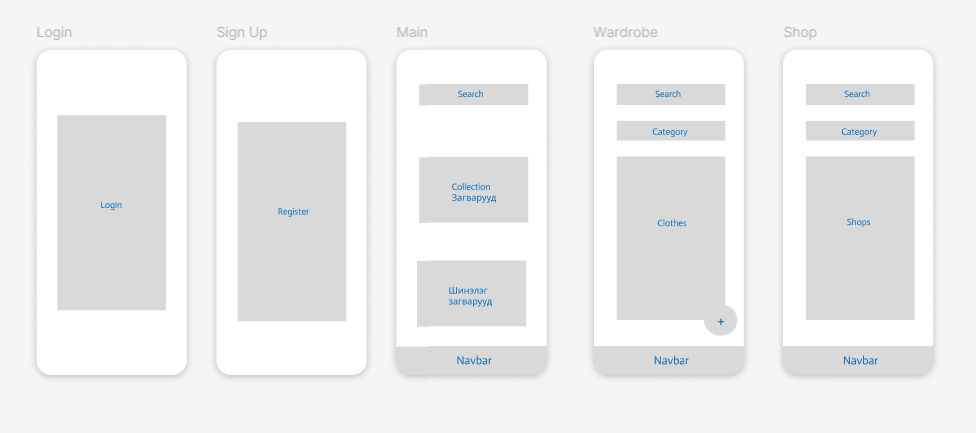
\includegraphics[width=\textwidth]{figures/Capture1.PNG}
    \label{}
\end{figure}
\paragraph{} SignUp буюу Register хэсэгт өөрийн бүртгэлийг үүсгэх бөгөөд системд нэвтрэхдээ Login дэлгэцээс нэвтэрнэ. Нэвтэрсний дараа Main дэлгэцээс дараах зүйлсийг харж болох бөгөөд доор байрлах navigator bar аас системийн бусад хэсгүүд рүү орно.Wardrobe хэсэгт өөрийн хувцаснуудыг хайх болон хувцас нэмэх хэсэг байна. Shop хэсэгт хувцас хайх хэсэг болон category хэсэгүүд байрлана.
\begin{figure}[H]
    \centering
    \caption{Profile, AI, Clothing, Clothing Idea дэлгэцүүд }
    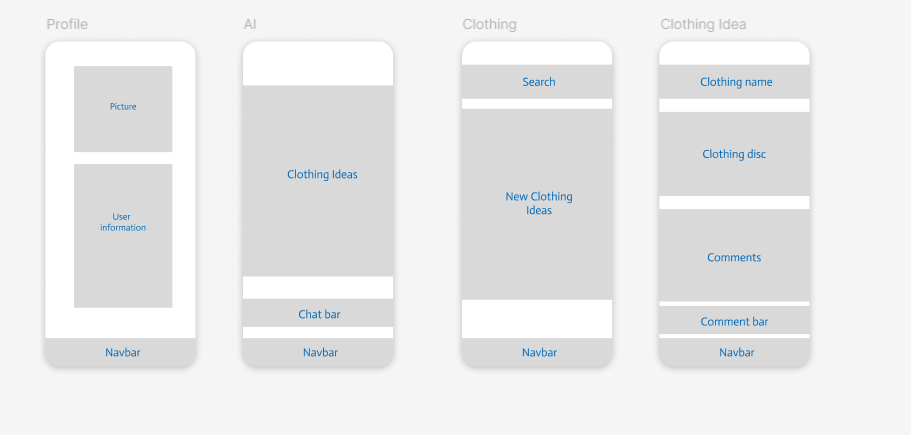
\includegraphics[width=\textwidth]{figures/Capture2.PNG}
    \label{}
\end{figure}
\paragraph{} Profile хэсэгт хэрэглэгчийн зураг болон хувийн мэдээллүүд байрлах болно. АI хэсэгт хэрэглэгч нь хиймэл оюун ухаантай мэдээллээ солилцож шинэлэг хувцаслалтуудыг үүсгэх боломжтой. Clothing хэсэг хэрэглэгчийн авсан хувцаслалтууд байх бөгөөд хэрэглэгч тэдгээр хувцаслалтууд руу ороход Clothing Idea дэлгэц рүү шилжинэ.


